\chapter{Komunikacja między wątkowa w środowisku ROS}

Komunikacja między minikomputerem pokładowym, a zdalnym komputerem została zrealizowana w oparciu o komunikację między wątkową w środowisku ROS. Wykorzystana wersja systemu to ROS Kinetic Kame, która jest kompatybilna z systemem Ubuntu 16.04 Xenial.

Komunikacja przebiega przez sieć wi-fi. W tym celu w pliku \textit{~/.bashrc} zostały zdefiniowane adresy IP wykorzystywane do komunikacji między wątkowej(Tabela \ref{ip_addres}). Umożliwiło to wykorzystanie tego samego rdzenia komunikacji. Węzły odpowiedzialne za generowanie wartości zadanej zostały zainicjalizowane na zdalnym komputerze, natomiast węzły odpowiedzialne za czujniki oraz połączenie z sterownikiem silnika zostały utworzone na minikomputerze pokładowym.



\begin{table}[h]
	\centering
	\caption{Definicja adresów wykorzystywanych przez ROS.}
	\label{ip_addres}
	\resizebox{\textwidth}{!}{%
		\begin{tabular}{c|c|c|}
			\cline{2-3}
			\textbf{}                              & \textbf{Zdalny komputer}             & \textbf{Platforma mobilna}           \\ \hline
			\multicolumn{1}{|c|}{ROS\_MASTER\_URI} & http://IP\_ZDALNEGO\_KOMPUTERA:11311 & http://IP\_ZDALNEGO\_KOMPUTERA:11311 \\ \hline
			\multicolumn{1}{|c|}{ROS\_HOSTNAME}    & IP\_ZDALNEGO\_KOMPUTERA              & IP\_PLATFORMY\_MOBILNEJ              \\ \hline
		\end{tabular}%
	}
\end{table}

\section{Komunikacja jednostki zdalnej}
Rdzeń komunikacji jest inicjalizowany na zdalnej jednostce, ponieważ posiada większą moc obliczeniową. Dodatkowo są na niej uruchamiane węzły odpowiedzialne za zadawanie sterowania, czyli prędkości kątowej i liniowej. Zostało to zrealizowane na trzy sposoby: z wykorzystaniem klawiatury, joysticka oraz MATLABA.

\subsection{Sterowanie w wykorzystaniem klawiatury}

Zadawanie prędkości liniowej i kątowej z wykorzystaniem klawiatury zostało zrealizowane przy pomocy biblioteki \textit{ros-kinetic-teleop-twist-keyboard}. Sterowanie odbywa się poprzez zwiększanie lub zmniejszanie prędkości i wybór, która z prędkości ma być aktywna(Rys. \ref{fig:klawiatura}). Publikowana wiadomość jest w formacie \textit{geometry\_msgs/Twist}, składa się ona z dwóch trójwymiarowych wektorów, jeden z nich odpowiada za prędkość liniową, a drugi za prędkość kątową.

\begin{figure}[ht]
	\centering
	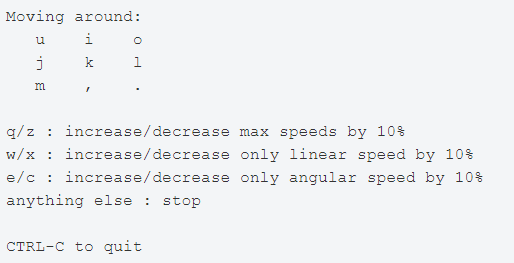
\includegraphics[scale=0.8]{keyboard.png}
	\caption{Sterowanie z wykorzystaniem klawiatury.}
	\label{fig:klawiatura}
\end{figure}

\subsection{Sterowanie z wykrorzystaniem joysticka}
Zostało zrealizowane z wykorzystaniem biblioteki \textit{ros-kinetic-joy}. Wychylenie lewej gałki powoduje zmianę wartości prędkości liniowej i kątowej w zależności od kierunku wychylenia. Wiadomość jest publikowana w formacie \textit{sensor\_msgs/Joy}. Składa się on z wektora określającego poziom wychylenia gałek oraz wektora ze stanem wszystkich dostępnych guzików. Informacja o przyciskach nie jest wykorzystywana, lecz pozwala na rozbudowanie sterowania z wykorzystaniem joysticka o dodatkowe funkcjonalności. 

\subsection{Sterowanie z wykorzystaniem środowiska MATLAB}

Środowisko MATLAB oferuje pakiet \textit{ROS Toolbox}, który pozwala na współprace z system ROS. Zawiera on gotowe funkcje odpowiedzialne za inicjalizację węzła oraz publikowanie i subskrypcję tematu. Dodatkowo obsługuje formaty danych wykorzystywane w komunikacji między wątkowej.  ROS Toolbox posiada także rozszerzenie do Simulink, dzięki któremu dostępne są nowe bloki umożliwiające obsługę ROS.

Sterowanie z wykorzystaniem MATLABa opiera się na stworzeniu węzła w tym środowisku. Program umożliwia stworzenie skryptu, w którym można zadawać sterowanie poprzez publikowanie wiadomości. Wykorzystany format to \textit{geometry\_msgs/Twist}. Takie rozwiązanie posiada przewagę nad dwoma poprzednimi, ponieważ możliwe jest generowanie sterowania na podstawie odczytów z czujników, które węzeł subskrybuje. Pozwala to na stworzenie algorytmów, generujących trajektorię poruszania się robota. Dodatkowo węzeł stworzony w MATLABie pozwala w prosty sposób zmieniać nastawy regulatora wykorzystywanego przez sterownik silników.

\section{Komunikacja jednostki pokładowej}

Minikomputer wbudowany łączy się z rdzeniem uruchomionym na jednostce zdalnej. Odpowiada on za uruchomienie trzech węzłów odpowiadających za system wizyjny, lidar oraz sterownik silników. Węzły są inicjalizowane przy pomocy skryptu napisanego w języku python. 

\subsection{Komunikacja systemu wizyjnego}

Wykorzystanym systemem wizyjnym jest kamera RealSense R200, która jest kompatybilna z minikomputerem pokładowym UpBoard. Komunikacja między wątkowa ROS została przeprowadzona w oparciu o bibliotekę \textit{ros-kinetic-realsense-camera}. Umożliwia ona inicjalizację węzła, który publikuje wiadomości o odczytach z kamery. Wiadomości są publikowane w wielu tematach, odpowiedzialnych za kalibrację, obraz w formacie RGB, głębokość obrazu stworzoną poprzez wykorzystanie dwóch kamer, oraz obraz w podczerwieni. 

\subsection{Komunikacja Lidaru}

Komunikacja z laserowym skanerem została przeprowadzona z wykorzystaniem biblioteki \textit{rplidar\_ros}. Pozwala ona na inicjalizację węzła odpowiedzialnego za lidar. Publikuje on w temacie \textit{scan} wiadomość w formacie 
\textit{sensor\_msgs/LaserScan}. Pozwala to na stworzenie mapy punktów, które zostały zeskanowane przez laser. W połączeniu z jednostką inercyjną lidar umożliwia mapowanie otoczenia robota. 


\subsection{Komunikacja sterownika silnika}

Komunikacja między wątkowa sterownika silnika jest możliwa dzięki bibliotece \textit{roserial}. Pozwala ona na inicjalizację własnego węzła przez wykorzystany miko kontroler STM32. Połączenie odbywa się  z prędkością transmisji wynoszącą 57600 i wykorzystuje port USB \textit{/dev/ttyACM0}.

W oprogramowaniu mikro kontrolera został utworzony węzeł, który pozwala na subskrybowanie tematów i publikację wiadomości.
\subsubsection{Tematy subskrybowane przez sterownik silników}

Subskrypcja tematów pozwala na uzyskanie dostępu do wiadomości, która pojawiła się na obserwowanym temacie. W momencie pojawienia się nowej wiadomości wywołana zostaje funkcja przypisana do danego tematu. Wewnątrz takiej funkcji znajduje się kod programu odpowiedzialny za  przypisanie wiadomości do zmiennych, skąd mogą być wykorzystane w programie. 

Głównymi tematami subskrybowanymi przez sterownik silników są tematy związane z zadawaniem prędkości liniowej i kątowej(Tabela \ref{subscribers}). Dodatkowo subskrybowany jest temat zawierający nastawy regulatora PID, pozwala to w łatwy sposób nimi manipulować.  

% Please add the following required packages to your document preamble:
% \usepackage{graphicx}
\begin{table}[h]
	\centering
	\caption{Tematy subskrybowane przez sterownik silników..}
	\label{subscribers}
	\resizebox{\textwidth}{!}{%
		\begin{tabular}{|c|c|c|}
			\hline
			\textbf{Temat} & \textbf{Opis wiadomości}                                   & \textbf{Format wiadomości}  \\ \hline
			cmd\_vel       & prędkość liniowa i kątowa zadana poprzez konsolę systemową & geometry\_msgs/Twist        \\ \hline
			joy            & prędkość liniowa i kątowa zadana poprzez joystick          & sensor\_msgs/Joy            \\ \hline
			mat\_vel       & prędkość liniowa i kątowa zadana poprzez środowisko MATLAB & geometry\_msgs/Twist        \\ \hline
			pid\_param     & nastawy regulatora PID                                     & std\_msgs/Float32MultiArray \\ \hline
		\end{tabular}%
	}
\end{table}




\subsubsection{Wiadomości publikowane przez sterownik silników }

Sterownik silników publikuje także własne wiadomości na tematy subskrybowane przez zewnętrzne węzły. Podaje on informację o statusie silników, odczytach z czujników, a także wyznaczonej odometri(Tabela. \ref{publishers}). Stworzony został także temat pozwalający na detekcję błędów w oprogramowaniu. Tematy posiadają różną częstotliwość publikowania wiadomości, w zależności od ich zastosowania. 

% Please add the following required packages to your document preamble:
% \usepackage{graphicx}
\begin{table}[h]
	\centering
	\caption{Wiadomości publikowane  przez sterownik silników.}
	\label{publishers}
	\resizebox{\textwidth}{!}{%
		\begin{tabular}{|c|c|c|c|}
			\hline
			\textbf{Temat}    & \textbf{Opis wiadomości}                               & \textbf{Format wiadomości} & Częstotliwość nadawania {[}Hz{]} \\ \hline
			imu               & odczyt z czujników jednostki inercyjnej                & sensor\_msgs::Imu          & 200                              \\ \hline
			odom              & wartości wyznaczonej odometri robota                   & nav\_msgs::Odometry        & 200                              \\ \hline
			imu\_state        & stan jednostki inercyjnej, wartość ujemna oznacza błąd & std\_msgs::Int32           & 30                               \\ \hline
			l\_engines\_state & status silników po lewej stronie, '1' oznacza błąd     & std\_msgs::Bool            & 30                               \\ \hline
			r\_engines\_state & status silników po prawej stronie, '1' oznacza błąd    & std\_msgs::Bool            & 30                               \\ \hline
			debug             & temat służący do debugowania programu sterownika       & geometry\_msgs::Twist      & 30                               \\ \hline
		\end{tabular}%
	}
\end{table}
